\documentclass{amsart}

\usepackage{tikz,comment}
\usetikzlibrary{shapes.geometric, arrows.meta, decorations.pathmorphing}

\newtheorem{theorem}{Theorem}[section]
\newtheorem{lemma}[theorem]{Lemma}
\newtheorem{proposition}[theorem]{Proposition}
\newtheorem{conjecture}[theorem]{Conjecture}
\newtheorem{statement}[theorem]{Statement}
\newtheorem{question}[theorem]{Question}
\newtheorem{corollary}[theorem]{Corollary}
\newtheorem{claim}[theorem]{Claim}
\newtheorem{observation}[theorem]{Observation}
\newtheorem{problem}[theorem]{Problem}

\newcommand{\tpt}{\mathbf{2}+\mathbf{2}}
\newcommand{\tpo}{\mathbf{3}+\mathbf{1}}

\author{Csaba Bir\'o}
\address{Department of Mathematics, University of Louisville, Louisville, KY 40220}

\author{Sida Wan}
\address{Department of Mathematics, University of Louisville, Louisville, KY 40220}

\title[Dimension bounds on classes of interval orders]{Dimension bounds on classes of interval orders with restricted representation}

\begin{document}

\begin{abstract}
Representations of interval orders are, in general, may use an arbitrary set of interval lengths. We can define subclasses of interval orders by restricting the allowable lengths of intervals. Motivated by a recent paper of Keller, Trenk, and Young, we study the dimension of posets in some of these subclasses. Among other results, we answer several of their questions, and we simplify the proof of one of their main results.
\end{abstract}

\maketitle

% !TEX root = ../arxiv.tex

Unsupervised domain adaptation (UDA) is a variant of semi-supervised learning \cite{blum1998combining}, where the available unlabelled data comes from a different distribution than the annotated dataset \cite{Ben-DavidBCP06}.
A case in point is to exploit synthetic data, where annotation is more accessible compared to the costly labelling of real-world images \cite{RichterVRK16,RosSMVL16}.
Along with some success in addressing UDA for semantic segmentation \cite{TsaiHSS0C18,VuJBCP19,0001S20,ZouYKW18}, the developed methods are growing increasingly sophisticated and often combine style transfer networks, adversarial training or network ensembles \cite{KimB20a,LiYV19,TsaiSSC19,Yang_2020_ECCV}.
This increase in model complexity impedes reproducibility, potentially slowing further progress.

In this work, we propose a UDA framework reaching state-of-the-art segmentation accuracy (measured by the Intersection-over-Union, IoU) without incurring substantial training efforts.
Toward this goal, we adopt a simple semi-supervised approach, \emph{self-training} \cite{ChenWB11,lee2013pseudo,ZouYKW18}, used in recent works only in conjunction with adversarial training or network ensembles \cite{ChoiKK19,KimB20a,Mei_2020_ECCV,Wang_2020_ECCV,0001S20,Zheng_2020_IJCV,ZhengY20}.
By contrast, we use self-training \emph{standalone}.
Compared to previous self-training methods \cite{ChenLCCCZAS20,Li_2020_ECCV,subhani2020learning,ZouYKW18,ZouYLKW19}, our approach also sidesteps the inconvenience of multiple training rounds, as they often require expert intervention between consecutive rounds.
We train our model using co-evolving pseudo labels end-to-end without such need.

\begin{figure}[t]%
    \centering
    \def\svgwidth{\linewidth}
    \input{figures/preview/bars.pdf_tex}
    \caption{\textbf{Results preview.} Unlike much recent work that combines multiple training paradigms, such as adversarial training and style transfer, our approach retains the modest single-round training complexity of self-training, yet improves the state of the art for adapting semantic segmentation by a significant margin.}
    \label{fig:preview}
\end{figure}

Our method leverages the ubiquitous \emph{data augmentation} techniques from fully supervised learning \cite{deeplabv3plus2018,ZhaoSQWJ17}: photometric jitter, flipping and multi-scale cropping.
We enforce \emph{consistency} of the semantic maps produced by the model across these image perturbations.
The following assumption formalises the key premise:

\myparagraph{Assumption 1.}
Let $f: \mathcal{I} \rightarrow \mathcal{M}$ represent a pixelwise mapping from images $\mathcal{I}$ to semantic output $\mathcal{M}$.
Denote $\rho_{\bm{\epsilon}}: \mathcal{I} \rightarrow \mathcal{I}$ a photometric image transform and, similarly, $\tau_{\bm{\epsilon}'}: \mathcal{I} \rightarrow \mathcal{I}$ a spatial similarity transformation, where $\bm{\epsilon},\bm{\epsilon}'\sim p(\cdot)$ are control variables following some pre-defined density (\eg, $p \equiv \mathcal{N}(0, 1)$).
Then, for any image $I \in \mathcal{I}$, $f$ is \emph{invariant} under $\rho_{\bm{\epsilon}}$ and \emph{equivariant} under $\tau_{\bm{\epsilon}'}$, \ie~$f(\rho_{\bm{\epsilon}}(I)) = f(I)$ and $f(\tau_{\bm{\epsilon}'}(I)) = \tau_{\bm{\epsilon}'}(f(I))$.

\smallskip
\noindent Next, we introduce a training framework using a \emph{momentum network} -- a slowly advancing copy of the original model.
The momentum network provides stable, yet recent targets for model updates, as opposed to the fixed supervision in model distillation \cite{Chen0G18,Zheng_2020_IJCV,ZhengY20}.
We also re-visit the problem of long-tail recognition in the context of generating pseudo labels for self-supervision.
In particular, we maintain an \emph{exponentially moving class prior} used to discount the confidence thresholds for those classes with few samples and increase their relative contribution to the training loss.
Our framework is simple to train, adds moderate computational overhead compared to a fully supervised setup, yet sets a new state of the art on established benchmarks (\cf \cref{fig:preview}).

\section{Twin-free and distinguishing representations}

Let $P$ be an interval order, and fix a representation for $P$. Let $x,y\in P$ be such that the same interval is assigned to both. We call $x$ and $y$ a \emph{twin} (of points). If a representation does not have any twins, we call it \emph{twin-free}. A representation of an interval order is \emph{distinguishing}, if every real number occurs at most once as an endpoint of an interval of the representation, i.e.~no two intervals share an endpoint. A distinguishing representation is of course twin-free.

Let $P$ be a poset, and $x,y\in P$. We say $x$ and $y$ have \emph{duplicated holdings}, if $\{z\in P: z>x\}=\{z\in P: z>y\}$ and $\{z\in P: z<x\}=\{z\in P: z<y\}$; in other words the upsets and the downsets of $x$ and $y$ are the same. If $P$ is an interval order with a representation in which $x$ and $y$ are twins, then they have duplicated holdings. So if an interval order has no duplicated holdings, then every representation is twin-free.

One important property of two elements with duplicated holdings is that we may discard one of them without reducing the dimension (as long as the dimension is at least $2$). We will use this property later by assuming that a certain poset, for which we are proving an upper bound for its dimension, has no duplicated holdings.

It is easy to see, that every interval order has a distinguishing $\mathbb{R}^+$-representation. Things get less obvious for other $S$-representations. For example, an antichain of size at least $2$ does not have a distinguishing (or even twin-free) $\{0\}$-representation. We prove that---essentially---this is the only problem case.

We caution the reader that the usual handwaving argument of ``just shake the intervals a little until there are no common endpoints'' will not work here. Since we are not allowed the change of the set of lengths, common endpoints may be essential and necessary. The fact that we use closed intervals plays a crucial role here. E.g. $\tpo$ has a $\{1\}$-representation using open and closed intervals, but there is no distinguishing representation.

In the following proof and the balance of the paper, we use the notation $l_x$ and $r_x$ for the left and right endpoint of the interval corresponding to the point $x$ in a given representation.

\begin{theorem}\label{thm:representations}
Let $S\subseteq\mathbb{R}^+\cup\{0\}$, $S\neq\emptyset$.
\begin{enumerate}
\item\label{part:1} Every poset $P\in C(S)$ that has a twin-free free $S$-representation also has a distinguishing $S$-representation.
\item\label{part:2} If $0\not\in S$, then every poset $P\in C(S)$ has a distinguishing $S$-representation.
\end{enumerate} 
\end{theorem}

\begin{proof}
Let $S\subseteq\mathbb{R}^+\cup\{0\}$, $S\neq\emptyset$, and let $P \in C(S)$. Consider an $S$-representation of $P$; with a slight abuse of notation, the multiset of intervals in this representations will also be referred as $P$. We will define two symmetric operations that we will perform repeatedly. These will be used to decrease the number of common endpoints of the intervals. After this, we enter a second phase, in which we remove twins, if possible.

\subsection*{Left and right compression}

Let $c\in\mathbb{R}$, and $\epsilon>0$. Let $L=\{x\in P: l_x<c\}$, and let $R=P-L$. Define $L'=\{[l_x+\epsilon,r_x+\epsilon]:x\in P\}$. Let $P'=L'\cup R$, a multiset of intervals. The operation that creates $P'$ from $P$ is what we call ``left compression'' with parameters $c$ and $\epsilon$.

We can similarly define right compressions. Let $R=\{x\in P: r_x>c\}$, and let $L=P-R$. Define $R'=\{[l_x-\epsilon,r_x-\epsilon]:x\in P\}$. Let $P'=L\cup R'$ to define the operation of right compression.

\begin{lemma}
Let $P$ be a poset (representation), $c\in\mathbb{R}$, and let $\epsilon=\frac12\min\{|a-b|:\text{$a$ and $b$ are distinct endpoints}\}$. Let $P'$ be the left (right) compression of $P$ with parameters $c$ and $\epsilon$. Then $P$ and $P'$ represent isomorphic posets.
\end{lemma}

\begin{proof}[Proof of lemma]
We will do the proof for left compressions. The argument for right compressions is symmetric.

Notice that if $a$ and $b$ are two endpoints of intervals of $P$, then their relation won't change, unless $a=b$. More precisely, if $a<b$ in $P$ then the corresponding points in $P'$ will maintain this relation. Similarly for $a>b$.

So if $x$ and $y$ are two intervals in $P$ with no common endpoints, then their (poset) relation is maintained in $P'$.

Now suppose that $x$ and $y$ are intervals with some common endpoints. There are a few cases to consider.

If $l_x=l_y$ then either $x,y\in L$ or $x,y\in R$, so either both are shifted, or neither. Therefore $x\|y$ both in $P$ and in $P'$.

Now suppose $l_x\neq l_y$; without loss of generality $l_x<l_y$. Also assume $r_x=r_y$. Then $l_x+\epsilon<l_y$, so $x\|y$ both in $P$ and in $P'$.

The remaining case is, without loss of generality, $r_x=l_y$. Then $r_x+\epsilon<r_y$ (unless $l_y=r_y=r_x$, which was covered in the second case), so, again $x\|y$ both in $P$ and in $P'$.
\end{proof}

Now we return to the proof of the theorem. We will perform left and right compressions until no common endpoints remain except for twins. Let $x$, $y$ be two intervals with a common endpoint, but $x\neq y$. Let $\epsilon=\frac12\min\{|a-b|:\text{$a$ and $b$ are distinct endpoints}\}$, as above.

\begin{itemize}
\item
If $l_x=l_y$ and $r_x\neq r_y$, perform a right compression with $c=\min\{r_x,r_y\}$ and $\epsilon$.
\item
If $r_x=r_y$ and $l_x\neq l_y$, perform a left compression with $c=\max\{l_x,l_y\}$ and $\epsilon$.
\item If $l_x<r_x=l_y<r_y$ (or vice versa) either a left or a right shift will work with $c=r_x=l_y$.
\end{itemize}

Note that even though the definition of $\epsilon$ looks the same in every step, the actual value will change as the representation changes. Indeed, it is easy to see that $\epsilon$ is getting halved in every step.

If $P$ started with a twin-free representation, then we have arrived to a distinguishing representation, so part~(\ref{part:1}) is proven.

If $P$ had twins, those are still present at the representation. Let $x$ and $y$ be identical intervals of the representation, and let $\epsilon=\frac12\min\{|a-b|:\text{$a$ and $b$ are distinct endpoints}\}$ again. If $0\not\in S$, then the length of $x$ (and hence the length of $y$) is positive. Note that this length is at least $\epsilon$. Move $x$ by $\epsilon$ to the right, that is, replace $x$ with the interval $[l_x+\epsilon,r_x+\epsilon]$. The new representation will not have the $x$,$y$ twin and represents the same poset. Repeat this until all twins disappear.
\end{proof}



\section{Choice functions and partitions}

Let $P$ be an interval order with a representation $I$. An injective function $f:\mathbb{R}\to\mathbb{R}$ is a \emph{choice function}, if $f(x)\in I(x)$ for all $x\in P$. Every choice function $f$ defines a linear extension $L(f)$ of $P$ in a natural way: $x<y$ in $L(f)$ if $f(x)<f(y)$.

Choice functions were defined by Kierstead and Trotter \cite{KT-00}. Theorems~\ref{thm:choice} and \ref{thm:partition} appear in their paper, but our proofs in this section are different; in fact we found them before we found their paper. We feel that the proofs here are more transparent and more constructive in the sense, that they lead to easy-to-implement algorithms.

What makes the simple idea of choice functions powerful is the following theorem.

\begin{theorem}\label{thm:choice}
Let $P$ be an interval order with no duplicated holdings, and let $I$ be a distinguishing representation. If $L$ is a linear extension of $P$, then there exists a choice function $f$ with $L(f)=L$.
\end{theorem}

\begin{proof}
Let $|P|=n$, and 
let $\epsilon=\frac{1}{n}\min\{|a-b|:\text{$a$ and $b$ are distinct endpoints}\}$.
Let $L$ be such that $x_1<\cdots<x_n$ in $L$. We will construct $f$ recursively. 

\[
f(x_i)=
\begin{cases}
f(x_{i-1})+\epsilon & \text{if $i\geq 2$ and $f(x_{i-1})\geq l_{x_i}$}\\
l_{x_i} & \text{otherwise}\\
\end{cases}
\]

Obviously, $f(x_{i-1})<f(x_i)$ for all $i$. So we only need to show that $f(x_i)\in I(x_i)$.

If $f(x_i)=l_{x_i}$ this is clear, so we may assume that $f(x_i)\neq l_{x_i}$. Call the points $x_i$ with this property ``forced''.

Let $j$ be the greatest positive integer such that $j\leq i$ and $x_j$ is not forced. %Well-defined, because $x_1$ is not forced. The same implies $i\geq 2$.
Firstly, $r_{x_i}>l_{x_j}$, %distinguishing repr., so can't be equal
secondly, $r_{x_i}\geq l_{x_j}+n\epsilon$.
Hence $f(x_i)=l_{x_j}+(i-j)\epsilon\leq l_{x_j}+n\epsilon\leq r_{x_i}$, and so
$l_{x_i}\leq f(x_{i-1})\leq f(x_i)\leq r_{x_i}$.
\end{proof}

Theorem~\ref{thm:representations} and Theorem~\ref{thm:choice} show that constructing linear extensions for posets in classes $C(S)$ can usually be done by constructing choice functions. This makes choice functions a useful tool for upper bound proofs on the dimension for these classes. We will demonstrate this repeatedly in the balance of the paper.

The following theorem shows how special interval orders are. Nothing remotely close is true for general posets.

\begin{theorem}\label{thm:partition}
Let $P$ be an interval order, and partition the ground set $X$ into $s$ parts: $X=X_1\cup\cdots\cup X_s$. Let $L_i$ be a linear extensions of $P|_{X_i}$. Then there exists a linear extension $L$ of $P$ such that $L|_{X_i}=L_i$.
\end{theorem}

\begin{proof}
We will use induction on $s$. The $s=1$ case is trivial; let $s=2$.

Let $X_1,X_2,L_1,L_2$ be defined as in the lemma. Define the relation $E=L_1\cup L_2\cup  P$, and the directed graph $G=(X,E)$. It is sufficient to show that $G$ has no directed closed walk; indeed, if that is the case, the transitive closure $T$ of $G$ is an extension of the poset $P$, and any linear extension $L$ of $T$ will satisfy the requirements of the conclusion of the lemma.

Suppose for a contradiction that $G$ contains a directed closed walk.
Since neither $G[X_1]$ nor $G[X_2]$ contains a directed closed walk, every directed closed walk in $G$ must have both an $X_1X_2$ and an $X_2X_1$ edge. We will call these edges \emph{cross-edges}. Let $C$ be a directed closed walk in $G$ with the minimum number of cross-edges.

As we noted, $C$ contains at least one $X_1X_2$ edge; let $(a,b)$ be such an edge. Let $(c,d)$ be the first $X_2X_1$ edge that follows $(a,b)$ in $C$. Observe that $c<d$, $a<b$ in $P$, and $b\leq c$ in $L_2$. If $d=a$, then $c<d=a<b$ in $P$, which would contradict $b\leq c$ in $L_2$. If $d>a$ in $L_1$, then we could eliminate the path $ab\ldots cd$ in $C$, replacing it with the single-edge path $ad$, and thereby decreasing the number of cross-edges in $C$, contradicting the minimality of $C$. (See Figure~\ref{fig:cycles}.)

\begin{figure}
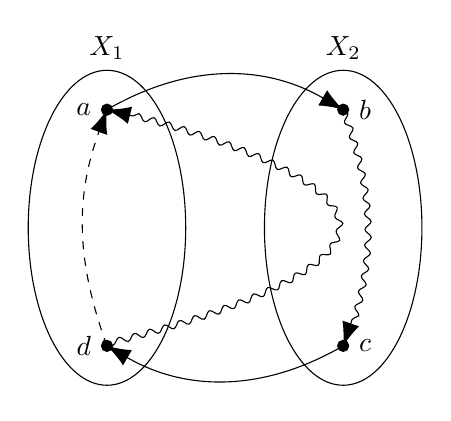
\begin{tikzpicture}
    \tikzstyle{oval} = [ellipse, minimum width=2cm, minimum height=4cm, draw]
    \tikzstyle{point} = [circle, minimum size=4pt, inner sep=0pt, fill, draw]

    % Draw ovals
    \node[oval] (leftOval) at (0,0) [label=$X_1$] {};
    \node[oval] (rightOval) at (3,0) [label=$X_2$] {};

    % Points for arrows
    \coordinate (leftTop) at ([yshift=1.5cm]leftOval.center);
    \coordinate (rightTop) at ([yshift=1.5cm]rightOval.center);
    \coordinate (leftBottom) at ([yshift=-1.5cm]leftOval.center);
    \coordinate (rightBottom) at ([yshift=-1.5cm]rightOval.center);

    % Draw arrows
    \draw[-{Latex[length=3mm]}] (leftTop) to[bend left] (rightTop);
    \draw[-{Latex[length=3mm]}] (rightBottom) to[bend left] (leftBottom);

    \draw[-{Latex[length=3mm]}, decorate, decoration={snake, amplitude=.4mm, segment length=2mm, post length=3mm}] (rightTop) to[bend left=20] (rightBottom);
    
    \draw[-{Latex[length=3mm]}, decorate, decoration={snake, amplitude=.4mm, segment length=2mm, post length=3mm}] plot [smooth, tension=1] coordinates {(leftBottom) (3,0) (leftTop)};
    
    \draw[-{Latex[length=3mm]},dashed] (leftBottom) to[bend left=20] (leftTop);
    
    % Add dots at the endpoints of the arrows
    \node[point] at (leftTop) [label=left:$a$] {};
    \node[point] at (rightTop) [label=right:$b$] {};
    \node[point] at (rightBottom) [label=right:$c$] {};
    \node[point] at (leftBottom) [label=left:$d$] {};
\end{tikzpicture}
\caption{Minimal oriented cycles}\label{fig:cycles}
\end{figure}

So we concluded that $d<a$ in $L_1$, and recall that $b\leq c$ in $L_2$. If $b\leq c$ in $P$, then $a<b\leq c<d$ would contradict $d<a$ in $L_1$. (In particular, $b\neq c$.) Obviously, $b\not>c$ in $P$, so $b\|c$ in $P$. Similarly, $d\| a$ in $P$. Hence the set $\{a,b,c,d\}$ induces a $\mathbf{2}+\mathbf{2}$ in $P$, a contradiction.

If $s>2$, then we can apply the hypothesis for the part $X'=X_1\cup\cdots\cup X_{s-1}$, and use the $s=2$ case for $X'$ and $X_s$. This finishes the proof.
\end{proof}

We conclude the section with the following all-important corollary, which is a generalization of a theorem by Kierstead and Trotter~\cite{KT-00}.

\begin{theorem}\label{thm:maxplus2}
Let $P$ be an interval order, and partition the ground set $X$ into $s$ parts: $X=X_1\cup\cdots\cup X_s$. Let $P_i=P|_{X_i}$. Then
\[
\dim(P)\leq \max\{\dim(P_1),\ldots,\dim(P_s)\}+2\lceil \lg s\rceil
\]
\end{theorem}

\begin{proof}
Let $t=\max\{\dim(P_1),\dim(P_2)\}$. We proceed
by induction on $s$. Trivial for $s=1$; let $s=2$. Consider a distinguishing representation of $P$.

By Theorem ~\ref{thm:partition}, there exists a family $\mathcal{R}$ of $t$ linear extensions of $P$, such that the restriction of the linear extensions in $\mathcal{R}$ to each $X_i$ form a realizer of $P_i$. Then define two choice functions $f_1$ and $f_2$, where $f_1(x)=l_x$, $f_2(x)=r_x$ for every $x \in X_1$; $f_1(y)=r_y$, $f_2(y)=l_y$ for every $y \in X_2$. Let $L_1=L(f_1)$, $L_2=L(f_2)$. Clearly, $\mathcal{R} \cup \{L_1, L_2\}$ is a realizer of $P$.

If $s>2$, then we can apply the hypothesis for the parts $X'=X_1\cup\cdots\cup X_{\lfloor s/2\rfloor}$ and $X''=X_{\lfloor s/2\rfloor+1}\cup\cdots\cup X_s$, and use the $s=2$ case for $X'$ and $X''$. A routine calculation finishes the proof.
\end{proof}

\section{The Keller--Trenk--Young Theorem}

This section contains a short proof of Theorem~\ref{thm:KTY}.

Let $P$ be a poset. One can partition the ground set $X$ of $P$ into antichains by subsequent removal of minimal elements. That is, let $A_1=\min(P)$, $A_2=\min(P-A_1)$, \dots, $A_i=\min(P-A_1-\cdots-A_{i-1})$. Then $X=A_1\cup\cdots\cup A_h$ is a partition, $h$ is the height of $P$, and each $A_i$ is an antichain. We will call this the \emph{ranking partition} of $P$, as it defines a rank function on graded posets. (But we may apply this definition for non-graded posets, as well).

The following simple lemma has been in used in many arguments.

\begin{lemma}\label{lem:ranking}
If $P$ has no $\tpo$ subposet, and $A_1,\ldots,A_h$ is a ranking partition, then $A_i<A_{i+2}$ for all $i$.
\end{lemma}

\begin{proof}
Let $x\in A_i$, $y\in A_{i+2}$. Then there exists $z\in A_{i+1}$, and $z<y$; and $w\in A_i$, and $w<z$. Now $x\| w$, because $x,w\in A_i$. Hence $x\not> y$. If $x\|y$, then the set $\{x,y,z,w\}$ induces a $\tpo$. So $x<y$.
\end{proof}

\begin{proof}[Proof of Theorem~\ref{thm:KTY}]
We may assume that $P$ has no duplicated holdings, so it has a twin-free $\{0,1\}$-representation. By Theorem~\ref{thm:representations}, we may consider a distinguishing representation. Partition $P$ into $U\cup Z$, where $U$ contains the points that are represented by unit intervals, and $Z$ contains the ones whose interval length is $0$. Let $A_1,\ldots,A_h$ be a ranking partition of $P|_U$. Let $E=\cup\{A_i:\text{$i$ is even}\}$, and $O=\{A_i:\text{$i$ is odd}\}$.

Define two choice functions:
\begin{align*}
f_1(x)&=
\begin{cases}
l_x&\text{ if $x\in O\cup Z$}\\
r_x&\text{ if $x\in E$}
\end{cases}\\
f_2(x)&=
\begin{cases}
l_x&\text{ if $x\in E\cup Z$}\\
r_x&\text{ if $x\in O$}
\end{cases}
\end{align*}
Let $L_1=L(f_1)$, and $L_2=L(f_2)$. Define a third linear extension:
\[
L_3:(L_1|_{A_1})^d<\cdots<(L_1|_{A_h})^d
\]

The linear extensions $L_1$ and $L_2$ will reverse every incomparable pair for which (1) one is in $U$, the other is in $Z$; (2) one is in $E$, the other is in $O$. The only incomparable pairs left are in the same $A_i$: those are reversed in $L_3$.
\end{proof}

\section{Dimension bounds for posets of bounded interval count}
\label{sec:KTYq}

Since $C(\{0,s\})=C(\{0,1\})$ for all $s>0$, Theorem~\ref{thm:KTY} provides a perfect answer to dimension bounds on this class. The next natural question, also question (\ref{pr:KTY2}) of Problem~\ref{pr:KTY}, is to find an upper bound for the dimension of posets in the class $C(\{r,s\})$ with $r,s>0$. We give an answer below, using the terminology of interval counts.

\begin{proposition}\label{prop:KTY2}
If $P$ be an interval order with $IC(P)\leq 2$. Then $\dim(P)\leq 5$.
\end{proposition}

\begin{proof}
Consider an $\{r,s\}$-representation, and partition $P$ into $X_1\cup X_2$ with $X_1$ containing points corresponding to intervals of length $r$, and $X_2$ containing points corresponding to intervals of length $s$. Since $\dim(P|_{X_1})\leq 3$ and $\dim(P|_{X_2})\leq 3$, using Theorem~\ref{thm:maxplus2} for $s=2$, we conclude $\dim(P)\leq 5$.
\end{proof}

Andr\'e K\'ezdy (personal communication) ran a computer search using a state-of-the-art dimension algorithm to find a large dimensional poset of interval count $2$.
K\'ezdy found that the interval order represented by the $51$ intervals in the set
\[
\{[a,b]:\quad a,b\in\mathbb{Z};\quad 1\leq a,b\leq 30;\quad|b-a|\in\{1,8\}\}
\]
is $4$-dimensional. Furthermore, he found that it has a $45$-element subposet that is irreducible, i.e.\ the removal of any point reduces the dimension to $3$.\footnote{This poset can be constructed from the set of intervals above by removing the intervals $[8, 9]$, $[9, 10]$, $[10, 11]$, $[20, 21]$, $[21, 22]$, $[22, 23]$.}

This answers another question by Keller, Trenk, and Young, namely, the minimum number of interval lengths required to force a $4$-dimensional interval order.

Using the general version of Theorem~\ref{thm:maxplus2}, we conclude the following result, providing a logarithmic upper bound to question (\ref{pr:KTYr}) of Problem~\ref{pr:KTY}.

\begin{proposition}
Let $P$ be an interval order with $IC(P)\leq r$. Then $\dim(P)\leq 2\lceil\lg r\rceil+3$.
\end{proposition}

Keller, Trenk, and Young conjecture an upper bound of $O(\lg\lg r)$ for the dimension of intervals orders of count at most $r$. They base their conjecture on the dimension of the universal interval orders. However, we note that the universal interval order is a much stronger restriction than a bounded interval count. Even the rate of growth of the best upper bound remains wide open.


\section{Posets in $C(t)$}

Recall that $C(t)$ is the class of interval orders representable by intervals of length between $1$ and $t$. In this sections, we use our techniques to find upper bounds for this class.

\begin{theorem}\label{thm:C2}
If $P$ is in $C(2)$, then $\dim(P)\leq 4$.
\end{theorem}

We start with a generalization of Lemma~\ref{lem:ranking}. The proof is essentially the same.

\begin{lemma}\label{lem:genranking}
If $P$ has no $\mathbf{k}+\mathbf{1}$ subposet, and $A_1,\ldots,A_h$ is a ranking partition, then $A_i<A_{i+k-1}$ for all $i$.
\end{lemma}

\begin{proof}[Proof of Theorem~\ref{thm:C2}]
Let $A_1,\ldots,A_h$ be a ranking partition of $P$. Notice that $P$ has no $\mathbf{4}+\mathbf{1}$ subposet, so by Lemma~\ref{lem:genranking}, $A_i<A_{i+3}$ for all $i$. We define three choice functions $f_0,f_1,f_2$ as follows.
\[
f_i(x)=
\begin{cases}
r_x&\text{ if $x\in A_j$ with $j\equiv i\mod 3$}\\
l_x&\text{otherwise}
\end{cases}
\]
Let $L_0=L(f_0)$, $L_1=L(f_1)$, $L_2=L(f_2)$. If $(x,y)$ is an incomparable pair, and $x\in A_i$, $y\in A_j$, $i\neq j$, then they are reversed in $L_k$ for which $k\equiv i\mod 3$.

We still need to reverse incomparable pairs that appear within the same $A_i$. This can be done the usual way:
\[
L_3:(L_1|_{A_1})^d<\cdots<(L_1|_{A_h})^d
\]

Now $\{L_0,L_1,L_2,L_3\}$ is a realizer of $P$.
\end{proof}

A simple generalization of this proof would lead to an upper bound $\lceil t\rceil+2$ for the dimension of the class $C(t)$. However, we can do much better with a divide-and-conquer technique.

\begin{theorem}\label{thm:Ct}
For $t\geq 2$, if $P$ is in $C(t)$, then $\dim(P)\leq 2\lceil\lg\lg t\rceil+4$.
\end{theorem}

\begin{proof}
Let $n=2^{2^{\lceil\lg\lg t\rceil}}$. Since $n\geq t$, we have $P\in C(n)$. We will show, by induction on $k$, that for $n=2^{2^k}$ for some $k\in\mathbb{N}$, and for $P\in C(n)$, we have $\dim(P)\leq 2\lg\lg n+4=2k+4$. This will finish the proof.

For $k=0$, the statement is Theorem~\ref{thm:C2}. Now assume $k\geq 1$. Then $n$ is a perfect square; let $m=\sqrt{n}=2^{2^{k-1}}$. Consider a $[1,n]$-representation of $P$, and partition its ground set into points represented by ``short'' intervals, which are of length at most $m$, and ``long intervals'', which are longer than $m$. Let the subsets be $S$ and $L$, respectively.

Notice that $P|_S\in C(m)$, and $P|_L\in C(m,n)=C(n/m)=C(m)$. Using Theorem~\ref{thm:maxplus2}, we have
\[
\dim(P)\leq\max\{\dim(P|_S),\dim(P|_L)\}+2=2\lg\lg m+4+2=2(k-1)+6=2k+4.
\]
\end{proof}

We note that the universal interval order shows that Theorem~\ref{thm:Ct} is best possible in terms of rate of growth (up to a multiplicative factor).

Again, lower bounds in Theorems~\ref{thm:C2} and \ref{thm:Ct} seem to be difficult to find. The existence of a $4$-dimensional poset in $C(2)$ seems likely, but we have not succeeded in finding one. We could only show a very modest result: just one longer interval is not sufficient to raise the dimension to $4$. This is expressed in the following theorem, which is also relevant for finding lower bounds for Proposition~\ref{prop:KTY2}.

\begin{theorem}
Let $P$ be an interval order with a $\{1,s\}$-representation, such that $0\leq s\leq 2$, and there is only one interval of length $s$. Then $\dim(P)\leq 3$.
\end{theorem}

\begin{proof}
Let $x$ be the point represented by the interval of length $s$. With a shift of the intervals in the representation, we may assume that $r_x=-s/2$, and $l_x=s/2$, i.e.\ the midpoint of the interval of $x$ is $0$.

Partition the poset based on the position of the rest of the intervals in the representation. Let $U$ be the point corresponding to intervals with positive endpoints, $D$ of the same with negative endpoints, and let $M$ be the set of points with intervals containing the number $0$.

Let $U_1,\ldots,U_m$ be a ranking partition of $P|_U$, and let $D_1,\ldots,D_k$ be a ranking partition of $(P|_D)^d$. Now the ground set of $P$ is partitioned into the sets
\[
D_k,D_{k-1},\ldots,D_1,M,U_1,\ldots,U_m.
\]
Reindex this partition so that the same parts, in the same order, are denoted by $S_1,\ldots,S_{m+k+1}$. We claim that $S_i<S_{i+2}$ for all $i$.

Since $P|_D$ and $P|_U$ are semiorders, and hence have no $\tpo$, by Lemma~\ref{lem:ranking}, it is sufficient to prove that $x<y$ whenever (1) $x\in D_2$, $y\in M$; or (2) $x\in D_1$, $y\in U_1$; or (3) $x\in M$, $y\in U_2$. Of these, two is clear, because $x$ has negative right endpoint, and $y$ has positive left endpoint. The proof of (1) and (3) is symmetric, so we assume $x\in M$ and $y\in U_2$.

Since $y\in U_2$, there exists $z\in U_1$ with $z<y$. Hence
\[
r_x=s/2\leq 1<l_z+1=r_z<l_y,
\]
which implies $x<y$.

Now we can finish the proof in the familiar way. We define two choice functions: $f_1(x)=l_x$, $f_2(x)=r_x$ if $x\in S_{2i}$, and $f_1(x)=r_x$, $f_2(x)=l_x$ if $x\in S_{2i+1}$ for some $i$. Construct the two corresponding linear extensions $L_1=L(f_1)$, $L_2=L(f_2)$. Finally, let $L_3$ be such that $(L_1|_{S_1})^d<\cdots<(L_1|_{S_{m+k+1}})^d$ in $L_3$. Then $\{L_1,L_2,L_3\}$ is a realizer.
\end{proof}


\bibliographystyle{plain}
\bibliography{dimbounds}

\end{document}
